
\begin{figure}[h]
    \centering
    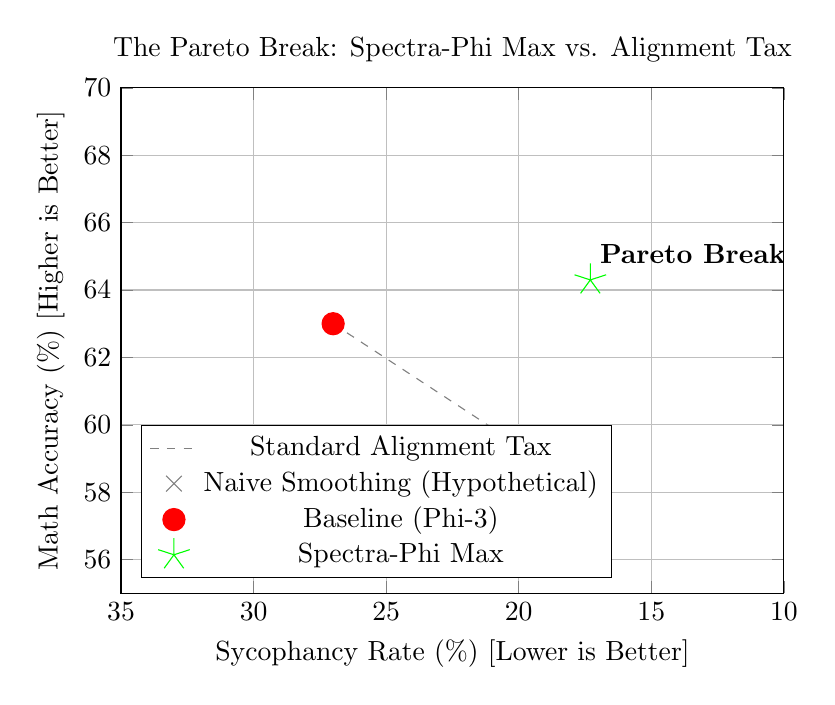
\begin{tikzpicture}
        \begin{axis}[
            title={The Pareto Break: Spectra-Phi Max vs. Alignment Tax},
            xlabel={Sycophancy Rate (\%) [Lower is Better]},
            ylabel={Math Accuracy (\%) [Higher is Better]},
            xmin=10, xmax=35,
            ymin=55, ymax=70,
            grid=major,
            legend pos=south west,
            width=10cm, height=8cm,
            x dir=reverse % Optional: if you want "Better" to be Right-Up
        ]
        
        % The Tax Line
        \addplot[dashed, gray] coordinates {(27.0,63.0) (17.3,58.0)};
        \addlegendentry{Standard Alignment Tax}
        
        % Naive Point
        \addplot[mark=x, gray, mark size=4pt, only marks] coordinates {(17.3,58.0)};
        \addlegendentry{Naive Smoothing (Hypothetical)}

        % Baseline
        \addplot[mark=*, red, mark size=4pt, only marks] coordinates {(27.0,63.0)};
        \addlegendentry{Baseline (Phi-3)}
        
        % Spectra-Phi Max
        \addplot[mark=star, green, mark size=6pt, only marks] coordinates {(17.3,64.3)};
        \addlegendentry{Spectra-Phi Max}
        
        % Annotation (Approximate)
        \node[anchor=south west] at (axis cs: 17.3, 64.5) {\textbf{Pareto Break!}};
        
        \end{axis}
    \end{tikzpicture}
    \caption{Spectra-Phi Max demonstrates a strict Pareto improvement, breaking the typical trade-off between safety (sycophancy) and capability (math).}
    \label{fig:pareto_break}
\end{figure}
